\chapter{Chain Rule and Trigonometric Derivatives}

% expansion:intuition — chapter overview tying ch03 to the differentiation toolkit started in ch02 and previewing what's still missing (chain rule for compositions)
Chapter 2 built the limit definition of the derivative and the elementary algebraic rules: constant, power, sum, constant-multiple, product, quotient, and the self-derivative property of the natural exponential. What we still cannot differentiate is a \emph{composition} \(f(g(x))\) when both pieces are non-trivial, and a class of functions --- the trigonometric functions and their inverses --- that we have used freely in earlier chapters but whose derivatives we have not computed. This chapter closes both gaps. We first compute \(d/dx \sin x\) and \(d/dx \cos x\) using a careful evaluation of \(\lim_{\theta \to 0} \sin \theta / \theta = 1\), then state and prove the \emph{chain rule} that handles compositions in full generality, and finally apply the chain rule to extract derivatives of \(\ln x\), \(\arcsin y\), and unusual exponentials such as \(x^{x}\). Together with the rigorous treatment of \(e^{x}\) and \(\ln x\) in Chapter 4, this completes the basic differentiation toolkit.

% expansion:summary — learning outcomes distilled from the manuscript. Verb-first per CONTENT_QUICKSTART.
\paragraph{By the end of this chapter, you will be able to:}
\begin{itemize}
    \item evaluate \(\displaystyle \lim_{\theta \to 0} \sin \theta / \theta = 1\) and \(\displaystyle \lim_{\theta \to 0} (1 - \cos \theta) / \theta = 0\) using the squeeze theorem and a sector-area inequality;
    \item differentiate \(\sin x\) and \(\cos x\) from first principles, and derive \(d/dx \tan x\) using the quotient rule;
    \item state the chain rule, recognise compositions in nested expressions, and apply it to differentiate \(f(g(x))\), \(f(g(h(x)))\), and similar nestings;
    \item use the chain rule together with implicit relations \(\sin(\arcsin y) = y\), \(e^{\ln x} = x\) to extract derivatives of inverse trigonometric functions, the natural logarithm, and exponentials with non-constant exponents.
\end{itemize}

\section{Derivatives of the Sine and Cosine Functions}\label{sec:sin-cos-derivatives}

% expansion:intuition — section opener motivating why we need trig derivatives now
The sine and cosine functions appeared in Chapter 1 (where we restricted them to define \(\arcsin\), \(\arccos\), and \(\arctan\)) and have been used freely since, but we have not yet computed their derivatives. The reason is that the difference quotient
\[
\frac{\sin(x + h) - \sin(x)}{h}
\]
does not simplify by the polynomial techniques of Chapter 2 --- we need a trigonometric identity to expand the numerator and a careful limit evaluation to make the denominator's \(h\) cancel. Both ingredients reduce to the single key fact
\[
\lim_{\theta \to 0} \frac{\sin \theta}{\theta} = 1,
\]
which is the heart of this section. We establish this limit using the squeeze theorem from \cref{sec:squeeze} and a sector-area inequality, then derive the derivatives of \(\sin x\) and \(\cos x\) almost immediately.

\subsection{The fundamental limit \texorpdfstring{$\lim_{\theta \to 0} \sin \theta / \theta = 1$}{lim sin theta / theta = 1}}

We begin with a geometric inequality involving a unit-circle sector and two triangles, valid for small positive angles \(\theta\).

\begin{figure}[H]
\centering
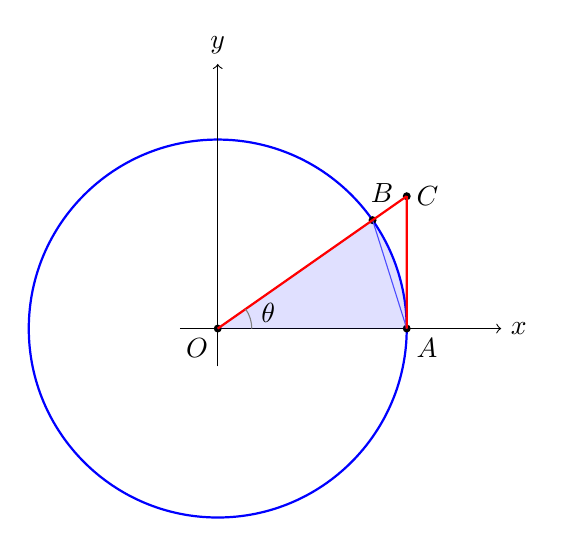
\begin{tikzpicture}[scale=2.4]
% Unit circle
\draw[blue, thick] (0,0) circle (1);
% x-axis
\draw[->] (-0.2,0) -- (1.5,0) node[right] {$x$};
\draw[->] (0,-0.2) -- (0,1.4) node[above] {$y$};
% Angle theta = 35 degrees
\def\angle{35}
% Point A on circle (right of theta=0)
\fill (1,0) circle (0.6pt);
\node[below right] at (1,0) {$A$};
% Point B on circle (at angle theta)
\coordinate (B) at ({cos(\angle)},{sin(\angle)});
\fill (B) circle (0.6pt);
\node[above] at ({cos(\angle)+0.05},{sin(\angle)+0.04}) {$B$};
% Point C above A on the tangent line at A
\coordinate (C) at (1,{tan(\angle)});
\fill (C) circle (0.6pt);
\node[right] at (C) {$C$};
% Origin
\fill (0,0) circle (0.6pt);
\node[below left] at (0,0) {$O$};
% Sector OAB shaded
\fill[blue, opacity=0.12] (0,0) -- (1,0) arc (0:\angle:1) -- cycle;
% Triangle OAB outlined
\draw[blue!70] (0,0) -- (B) -- (1,0);
% Triangle OAC outlined (right triangle)
\draw[red, thick] (1,0) -- (C);
\draw[red, thick] (0,0) -- (C);
% Theta angle arc
\draw[gray, thin] (0.18,0) arc (0:\angle:0.18);
\node at ({0.28*cos(\angle/2)},{0.28*sin(\angle/2)}) {$\theta$};
\end{tikzpicture}
\caption{Geometry for the bound \(\sin \theta \leq \theta \leq \tan \theta\). The blue circle is the unit circle; \(\overrightarrow{AC}\) is tangent to the circle at \(A\); the sector \(OAB\) sits between the inscribed triangle \(\triangle OAB\) (smaller) and the right triangle \(\triangle OAC\) (larger).}
\label{fig:sector-bound}
\end{figure}

\begin{lemma}\label{lem:sector-inequality}
For \(0 < \theta < \pi/2\),
\[
\sin \theta \leq \theta \leq \tan \theta,
\]
where \(\tan \theta = \sin \theta / \cos \theta\).
\end{lemma}

\begin{proof}
Refer to \cref{fig:sector-bound}. Working on the unit circle, with \(O\) the origin, \(A = (1, 0)\), \(B = (\cos \theta, \sin \theta)\), and \(C = (1, \tan \theta)\) the intersection of the tangent line at \(A\) with the ray \(\overrightarrow{OB}\):
\begin{itemize}
    \item the area of the inscribed triangle \(\triangle OAB\) is \(\tfrac{1}{2} \cdot 1 \cdot \sin \theta = \tfrac{1}{2} \sin \theta\);
    \item the area of the circular sector \(OAB\) is \(\tfrac{1}{2} \theta\) (a fraction \(\theta / (2\pi)\) of the disc area \(\pi\));
    \item the area of the right triangle \(\triangle OAC\) is \(\tfrac{1}{2} \cdot 1 \cdot \tan \theta = \tfrac{1}{2} \tan \theta\).
\end{itemize}
By the geometric containment \(\triangle OAB \subset \text{sector } OAB \subset \triangle OAC\), the corresponding areas obey
\[
\tfrac{1}{2} \sin \theta \;\leq\; \tfrac{1}{2} \theta \;\leq\; \tfrac{1}{2} \tan \theta.
\]
Multiplying by \(2\) gives the claimed inequality.
\end{proof}

% expansion:formula — the manuscript records this consequence but doesn't pull it out as a named corollary; promoting it makes the squeeze step that follows tidier
\begin{corollary}\label{cor:sin-theta-bound}
For \(0 < \lvert \theta \rvert < \pi/2\),
\[
\cos \theta \;\leq\; \frac{\sin \theta}{\theta} \;\leq\; 1,
\]
and consequently \(\lvert \sin \theta \rvert \leq \lvert \theta \rvert\) for every real \(\theta\).
\end{corollary}

\begin{proof}
For \(0 < \theta < \pi/2\), divide \cref{lem:sector-inequality} by \(\sin \theta > 0\):
\[
1 \;\leq\; \frac{\theta}{\sin \theta} \;\leq\; \frac{1}{\cos \theta},
\]
then take reciprocals (all positive), reversing inequality directions: \(\cos \theta \leq \sin \theta / \theta \leq 1\). For \(-\pi/2 < \theta < 0\), \(\sin \theta / \theta\) is even (numerator and denominator are both odd in \(\theta\)), so the same bound holds with \(\theta\) replaced by \(\lvert \theta \rvert\), and \(\cos \theta = \cos(-\theta)\) makes the lower bound symmetric too. The bound \(\lvert \sin \theta \rvert \leq \lvert \theta \rvert\) follows from \(\lvert \sin \theta \rvert / \lvert \theta \rvert \leq 1\) for \(0 < \lvert \theta \rvert < \pi/2\); for \(\lvert \theta \rvert \geq \pi/2 > 1 \geq \lvert \sin \theta \rvert\) the bound is trivial.
\end{proof}

\begin{theorem}\label{thm:sin-theta-over-theta}
\[
\lim_{\theta \to 0} \frac{\sin \theta}{\theta} = 1.
\]
\end{theorem}

\begin{proof}
The function \(\sin \theta / \theta\) is even in \(\theta\), so it suffices to take \(\theta > 0\). \Cref{cor:sin-theta-bound} sandwiches it between \(\cos \theta\) and \(1\):
\[
\cos \theta \;\leq\; \frac{\sin \theta}{\theta} \;\leq\; 1.
\]
The continuity of \(\cos\) at \(0\) (we prove this in \cref{prop:sin-cos-continuous} below) gives \(\lim_{\theta \to 0} \cos \theta = \cos 0 = 1\), and \(\lim_{\theta \to 0} 1 = 1\). The squeeze theorem (\cref{thm:squeeze}) then forces \(\lim_{\theta \to 0} \sin \theta / \theta = 1\).
\end{proof}

% expansion:caution — the dependence on cos continuity creates a circularity worry; flagging it is honest and prevents confusion
\begin{caution}
The proof of \cref{thm:sin-theta-over-theta} uses the continuity of \(\cos\) at \(0\), which we prove next as \cref{prop:sin-cos-continuous}. The argument is \emph{not} circular because \cref{prop:sin-cos-continuous}'s proof appeals only to the bound \(\lvert \sin \theta \rvert \leq \lvert \theta \rvert\) from \cref{cor:sin-theta-bound}, which in turn was established by pure geometry without using any limit. Reading the two proofs in order --- \cref{cor:sin-theta-bound} (geometric, no limits), \cref{prop:sin-cos-continuous} (uses the bound), \cref{thm:sin-theta-over-theta} (uses continuity) --- shows the dependency chain is acyclic.
\end{caution}

\subsection{Continuity of sine and cosine}

The sector-area bound \(\lvert \sin \theta \rvert \leq \lvert \theta \rvert\) is enough to prove that both \(\sin\) and \(\cos\) are continuous at every point.

\begin{proposition}\label{prop:sin-cos-continuous}\index{continuous!sine and cosine}
The functions \(\sin x\) and \(\cos x\) are continuous at every \(x \in \mathbb{R}\).
\end{proposition}

\begin{proof}
For sine: by the sum-to-product identity \(\sin(x + h) - \sin x = 2 \sin(h/2) \cos(x + h/2)\), so
\[
\bigl\lvert \sin(x + h) - \sin x \bigr\rvert
= 2 \bigl\lvert \sin(h/2) \bigr\rvert \cdot \bigl\lvert \cos(x + h/2) \bigr\rvert
\leq 2 \bigl\lvert \sin(h/2) \bigr\rvert
\leq 2 \cdot \frac{\lvert h \rvert}{2}
= \lvert h \rvert,
\]
where the first inequality uses \(\lvert \cos \rvert \leq 1\) and the second uses \cref{cor:sin-theta-bound}. Therefore \(\lvert \sin(x + h) - \sin x \rvert \to 0\) as \(h \to 0\), which is the definition of continuity at \(x\).

For cosine: by \(\cos x - \cos x_{0} = -2 \sin\bigl(\tfrac{x - x_{0}}{2}\bigr) \sin\bigl(\tfrac{x + x_{0}}{2}\bigr)\),
\[
\bigl\lvert \cos x - \cos x_{0} \bigr\rvert
\leq 2 \bigl\lvert \sin\bigl(\tfrac{x - x_{0}}{2}\bigr) \bigr\rvert
\leq \lvert x - x_{0} \rvert,
\]
which gives \(\lim_{x \to x_{0}} \cos x = \cos x_{0}\) directly.
\end{proof}

\subsection{The derivatives of sine and cosine}

With the limit \(\sin \theta / \theta \to 1\) and the continuity of \(\sin\) and \(\cos\) in hand, the derivatives drop out almost immediately.

\begin{theorem}\label{thm:derivative-sin}\index{sine!derivative}
\(\displaystyle \frac{d}{dx} \sin x = \cos x\) for every \(x \in \mathbb{R}\).
\end{theorem}

\begin{proof}
Apply the sum-to-product identity \(\sin(x + h) - \sin x = 2 \sin(h/2) \cos(x + h/2)\) to the difference quotient:
\[
\frac{\sin(x + h) - \sin x}{h}
= \frac{2 \sin(h/2) \cos(x + h/2)}{h}
= \frac{\sin(h/2)}{h/2} \cdot \cos\!\Bigl(x + \tfrac{h}{2}\Bigr).
\]
As \(h \to 0\), the first factor approaches \(1\) by \cref{thm:sin-theta-over-theta} (with \(\theta = h/2\)), and the second factor approaches \(\cos x\) by \cref{prop:sin-cos-continuous}. The product law for limits gives
\[
\frac{d}{dx} \sin x = \lim_{h \to 0} \frac{\sin(x + h) - \sin x}{h} = 1 \cdot \cos x = \cos x. \qedhere
\]
\end{proof}

\begin{theorem}\label{thm:derivative-cos}\index{cosine!derivative}
\(\displaystyle \frac{d}{dx} \cos x = -\sin x\) for every \(x \in \mathbb{R}\).
\end{theorem}

\begin{proof}
By the sum-to-product identity \(\cos(x + h) - \cos x = -2 \sin(h/2) \sin(x + h/2)\),
\[
\frac{\cos(x + h) - \cos x}{h}
= -\frac{\sin(h/2)}{h/2} \cdot \sin\!\Bigl(x + \tfrac{h}{2}\Bigr).
\]
Taking \(h \to 0\), the first factor again approaches \(1\) and the second approaches \(\sin x\), giving \(\cos'(x) = -\sin x\).
\end{proof}

% expansion:strategy [pass: enrichment] — distils the shared three-step template used in the proofs of \cref{thm:derivative-sin} and \cref{thm:derivative-cos}; Mode B's earlier audit flagged \S3.1's missing strategy box as a Mode C candidate, this fills it
\begin{strategy}[Differentiating $\sin$ or $\cos$ from first principles]
The proofs of \cref{thm:derivative-sin} and \cref{thm:derivative-cos} share a three-step template:
\begin{enumerate}
    \item \emph{Expand the difference quotient with a sum-to-product identity}, converting the difference into a product of one factor that depends only on \(h\) and one factor that depends on both \(x\) and \(h\). Sine uses \(\sin(x + h) - \sin x = 2 \sin(h/2) \cos(x + h/2)\); cosine uses \(\cos(x + h) - \cos x = -2 \sin(h/2) \sin(x + h/2)\).
    \item \emph{Factor so the \(h\)-only piece becomes the fundamental limit.} Divide by \(h\) and rewrite \(2 \sin(h/2)/h\) as \(\sin(h/2)/(h/2)\); this is the \(\sin \theta / \theta\) form (with \(\theta = h/2\)) that \cref{thm:sin-theta-over-theta} sends to \(1\).
    \item \emph{Send \(h \to 0\) using the limit-product law.} The \(\sin(h/2)/(h/2)\) factor approaches \(1\) by \cref{thm:sin-theta-over-theta}; the remaining \(\cos(x + h/2)\) or \(\sin(x + h/2)\) factor approaches \(\cos x\) or \(\sin x\) by \cref{prop:sin-cos-continuous}.
\end{enumerate}
The same template gives \(d/dx \tan x\) once one rewrites \(\tan x = \sin x / \cos x\) and applies the quotient rule (next), and it adapts to any difference quotient that a single trigonometric identity collapses into a product of an \(h\)-only piece and a continuous piece.
\end{strategy}

% expansion:formula — d/dx tan x is an immediate quotient-rule consequence; the manuscript doesn't include it but no calculus chapter on trig derivatives should omit it
\begin{corollary}\label{cor:derivative-tan}\index{tangent!derivative}
\(\displaystyle \frac{d}{dx} \tan x = \sec^{2} x\) wherever \(\cos x \neq 0\), where \(\sec x = 1/\cos x\).
\end{corollary}

\begin{proof}
Write \(\tan x = \sin x / \cos x\) and apply the quotient rule (\cref{thm:quotient-rule}):
\[
\frac{d}{dx} \tan x
= \frac{\cos x \cdot \cos x - \sin x \cdot (-\sin x)}{\cos^{2} x}
= \frac{\cos^{2} x + \sin^{2} x}{\cos^{2} x}
= \frac{1}{\cos^{2} x}
= \sec^{2} x. \qedhere
\]
\end{proof}

% expansion:caution — the chain-rule version of d/dx sin g(x) is the place students lose the inner derivative; flag it now so §3.2's chain rule isn't the first place they meet this trap
\begin{caution}
\Cref{thm:derivative-sin} and \cref{thm:derivative-cos} are stated for the bare functions \(\sin x\) and \(\cos x\). When the argument is a non-trivial expression --- \(\sin(x^{2})\), \(\cos(3x + 1)\), \(\sin(\ln x)\) --- the chain rule from \cref{sec:chain-rule} is required, and the inner derivative does \emph{not} cancel. The most common error is writing
\[
\frac{d}{dx} \sin(g(x)) = \cos(g(x)) \quad \text{(WRONG)}
\]
when the correct expression is \(\cos(g(x)) \cdot g'(x)\). Until the chain rule is in hand, only differentiate \(\sin x\) and \(\cos x\) directly, with \(x\) as the bare argument.
\end{caution}

% expansion:example — supplementary worked example using the trig derivatives in a product/quotient context. Manuscript doesn't include compound applications; without one the section feels abstract.
\begin{workedexample}
\begin{example}\label{ex:trig-product}
Differentiate \(p(x) = x^{2} \sin x\) and \(q(x) = \dfrac{\sin x}{x}\) (for \(x \neq 0\)).
\end{example}

\begin{solution}
By the product rule (\cref{thm:product-rule}):
\[
p'(x) = (x^{2})' \sin x + x^{2} (\sin x)' = 2x \sin x + x^{2} \cos x.
\]
By the quotient rule (\cref{thm:quotient-rule}):
\[
q'(x) = \frac{(\sin x)' \cdot x - \sin x \cdot (x)'}{x^{2}} = \frac{x \cos x - \sin x}{x^{2}}. \qedhere
\]
\end{solution}
\end{workedexample}

% expansion:summary — closing synthesis paragraph linking to §3.2
We can now differentiate every elementary function studied so far whose argument is a bare \(x\): polynomials, the natural exponential, sine, cosine, and (via the quotient rule) tangent. The next step is to handle compositions: once we know \(d/dx \sin x = \cos x\), what is \(d/dx \sin(x^{2})\)? The answer, as the caution above flagged, is not \(\cos(x^{2})\) alone; the inner function \(x^{2}\) contributes a factor of its own derivative. The chain rule, the subject of the next section, makes this precise.

\section{The Chain Rule}\label{sec:chain-rule}

% expansion:intuition — section opener pivoting from §3.1's "we cannot yet differentiate sin(g(x))"
The differentiation rules of \cref{sec:polynomial-exponential-derivatives,sec:product-quotient-rules} handle sums, differences, products, quotients, and constant multiples. The remaining elementary algebraic operation is \emph{composition}: given \(g\) differentiable at \(x\) and \(f\) differentiable at \(g(x)\), how do we differentiate the composite \(f(g(x))\)? The answer is the \emph{chain rule}, which says the slopes multiply: the rate of change of \(f \circ g\) at \(x\) equals the rate of change of \(f\) at the intermediate point \(g(x)\) times the rate of change of \(g\) at \(x\). This section states the chain rule, gives a proof using a slightly reframed definition of differentiability (the ``remainder form''), and then uses it to differentiate every composition we are likely to meet in this book.

\subsection{Two equivalent definitions of differentiability}

The standard definition of differentiability (\cref{def:derivative-at-a}) involves the limit of a difference quotient. An equivalent reformulation, more convenient for the chain-rule proof, expresses differentiability as a linear approximation with a small remainder.

\begin{definition}[Remainder form of differentiability]\label{def:differentiable-remainder}\index{differentiable!remainder form}\index{remainder form (differentiability)}
A function \(f\) is differentiable at \(x_{0}\) if there exists a real number \(m\) and a function \(R(h)\) such that
\[
f(x_{0} + h) = f(x_{0}) + m h + R(h),
\]
where the remainder \(R(h)\) satisfies
\[
\lim_{h \to 0} \frac{R(h)}{h} = 0.
\]

% expansion:intuition — Informally gloss for the remainder-form definition
\emph{Informally, \cref{def:differentiable-remainder} says that near \(x_{0}\), the function \(f\) is well approximated by the linear function \(h \mapsto f(x_{0}) + mh\), with an error \(R(h)\) that goes to \(0\) faster than \(h\) does. The slope \(m\) of this best linear approximation is \(f'(x_{0})\).}
\end{definition}

\begin{proposition}\label{prop:def-equivalence}
\Cref{def:differentiable-remainder} is equivalent to \cref{def:derivative-at-a}: \(f\) is differentiable at \(x_{0}\) under one definition if and only if it is differentiable under the other, and the constants match: \(m = f'(x_{0})\).
\end{proposition}

\begin{proof}
Suppose \(f\) is differentiable at \(x_{0}\) by \cref{def:derivative-at-a}, with derivative \(f'(x_{0})\). Define
\[
R(h) = f(x_{0} + h) - f(x_{0}) - f'(x_{0}) h.
\]
Then \(f(x_{0} + h) = f(x_{0}) + f'(x_{0}) h + R(h)\), and
\[
\frac{R(h)}{h} = \frac{f(x_{0} + h) - f(x_{0})}{h} - f'(x_{0}) \;\xrightarrow[h \to 0]{}\; f'(x_{0}) - f'(x_{0}) = 0.
\]
This is \cref{def:differentiable-remainder} with \(m = f'(x_{0})\).

Conversely, suppose \cref{def:differentiable-remainder} holds with constants \(m\) and \(R\). Then
\[
\frac{f(x_{0} + h) - f(x_{0})}{h} = \frac{m h + R(h)}{h} = m + \frac{R(h)}{h} \;\xrightarrow[h \to 0]{}\; m + 0 = m,
\]
so \(f\) is differentiable at \(x_{0}\) under \cref{def:derivative-at-a} with \(f'(x_{0}) = m\).
\end{proof}

% expansion:intuition — pedagogical motivation for why the remainder form is useful even though it's equivalent
\begin{remark}
The remainder form will not change any derivative calculation we have already done; it gives the same number for \(f'(x_{0})\) as before. Its advantage is for \emph{proofs}, particularly the chain-rule proof below: substituting the remainder-form expansion into a composition lets us track the contributions of \(f'\) and \(g'\) separately, with the remainders bookkept explicitly. We use \cref{def:differentiable-remainder} for the chain-rule proof and the standard \cref{def:derivative-at-a} everywhere else.
\end{remark}

\subsection{Statement of the chain rule}

\begin{theorem}[Chain rule]\label{thm:chain-rule}\index{chain rule}
Suppose \(g\) is differentiable at \(x_{0}\) and \(f\) is differentiable at \(y_{0} = g(x_{0})\). Then the composite \(p(x) = f(g(x))\) is differentiable at \(x_{0}\), with
\[
p'(x_{0}) = f'\!\bigl(g(x_{0})\bigr) \cdot g'(x_{0}).
\]
In Leibniz notation, with \(y = g(x)\) and \(z = f(y)\),
\[
\frac{dz}{dx} = \frac{dz}{dy} \cdot \frac{dy}{dx}.
\]
\end{theorem}

% expansion:caution — Leibniz form of chain rule is not fraction-cancellation, and treating it as such leads to subtler errors later (e.g. with partial derivatives). Worth flagging now.
\begin{caution}
The Leibniz form \(\dfrac{dz}{dx} = \dfrac{dz}{dy} \cdot \dfrac{dy}{dx}\) looks like a cancellation of \(dy\) in numerator and denominator, and that mnemonic is genuinely useful. But \(\dfrac{dz}{dy}\) and \(\dfrac{dy}{dx}\) are derivatives, not fractions of independently-defined quantities \(dz\) and \(dy\); the apparent cancellation is a consequence of the chain rule, not a derivation of it. Reasoning ``\(dy / dy = 1\)'' is informal at best; in multivariable settings (Calc III), the same notation will not satisfy the cancellation, and habits formed here lead to errors there.
\end{caution}

\subsection{Proof of the chain rule}

The proof uses the remainder form (\cref{def:differentiable-remainder}) for both \(g\) and \(f\) at the relevant points, then expands the composition.

\begin{proof}[Proof of \cref{thm:chain-rule}]
By \cref{def:differentiable-remainder} applied to \(g\) at \(x_{0}\),
\[
g(x_{0} + h) = g(x_{0}) + m_{1} h + R_{1}(h), \qquad m_{1} = g'(x_{0}), \quad \lim_{h \to 0} \frac{R_{1}(h)}{h} = 0,
\]
and applied to \(f\) at \(y_{0} = g(x_{0})\),
\[
f(y_{0} + k) = f(y_{0}) + m_{2} k + R_{2}(k), \qquad m_{2} = f'(y_{0}), \quad \lim_{k \to 0} \frac{R_{2}(k)}{k} = 0.
\]
Now expand \(p(x_{0} + h) = f(g(x_{0} + h))\). Substituting the first expansion into the second with \(k = m_{1} h + R_{1}(h)\),
\begin{aligneddisplay}
p(x_{0} + h) &= f\!\bigl(g(x_{0}) + m_{1} h + R_{1}(h)\bigr) \\
             &= f(y_{0}) + m_{2}\bigl[m_{1} h + R_{1}(h)\bigr] + R_{2}\bigl(m_{1} h + R_{1}(h)\bigr) \\
             &= p(x_{0}) + m_{1} m_{2} h + R_{3}(h),
\end{aligneddisplay}
where the remainder
\[
R_{3}(h) = m_{2} R_{1}(h) + R_{2}\!\bigl(m_{1} h + R_{1}(h)\bigr)
\]
collects every term that is not \(p(x_{0}) + m_{1} m_{2} h\). To finish the proof we must show \(R_{3}(h) / h \to 0\) as \(h \to 0\). The first piece is straightforward:
\[
\frac{m_{2} R_{1}(h)}{h} = m_{2} \cdot \frac{R_{1}(h)}{h} \to m_{2} \cdot 0 = 0.
\]
For the second piece, \(R_{2}(m_{1} h + R_{1}(h)) / h\), we argue as follows. Given \(\varepsilon > 0\), the limit \(R_{2}(k) / k \to 0\) gives some \(\delta > 0\) with \(\lvert R_{2}(k) / k \rvert < \varepsilon\) for \(0 < \lvert k \rvert < \delta\). Setting \(k = 0\) in the defining equation \(f(y_{0} + k) = f(y_{0}) + m_{2} k + R_{2}(k)\) yields \(R_{2}(0) = 0\), so the bound \(\lvert R_{2}(k) \rvert \leq \varepsilon \lvert k \rvert\) extends to \(\lvert k \rvert < \delta\) without the \(k \neq 0\) restriction (the case \(k = 0\) gives \(0 \leq \varepsilon \cdot 0\) trivially). The expression \(m_{1} h + R_{1}(h)\) approaches \(0\) as \(h \to 0\), so for \(h\) small enough, \(\lvert m_{1} h + R_{1}(h) \rvert < \delta\). Then
\[
\left\lvert \frac{R_{2}(m_{1} h + R_{1}(h))}{h} \right\rvert
\leq \frac{\lvert m_{1} h + R_{1}(h) \rvert}{\lvert h \rvert} \cdot \varepsilon
\leq \left(\lvert m_{1} \rvert + \frac{\lvert R_{1}(h) \rvert}{\lvert h \rvert}\right) \cdot \varepsilon.
\]
The factor in parentheses is bounded as \(h \to 0\) (the first term is constant, the second goes to \(0\)), so the entire expression is at most a constant times \(\varepsilon\). Since \(\varepsilon\) was arbitrary, \(R_{2}(m_{1} h + R_{1}(h)) / h \to 0\). Combining the two pieces, \(R_{3}(h) / h \to 0\), and \cref{def:differentiable-remainder} gives \(p\) differentiable at \(x_{0}\) with derivative \(m_{1} m_{2} = g'(x_{0}) f'(g(x_{0}))\), the chain rule.
\end{proof}

\subsection{Using the chain rule}

The chain rule turns differentiation of compositions into a routine procedure: identify the outer and inner functions, differentiate each at its own input, and multiply.

% expansion:strategy — the canonical chain-rule decomposition procedure; the highest-leverage skill in this section
\begin{strategy}[Differentiating \(f(g(x))\)]
To differentiate a composition:
\begin{enumerate}
    \item Identify the \emph{outer} function \(f\) and the \emph{inner} function \(g\) so that the expression is \(f(g(x))\). The outer function is the one that would be applied last if the expression were evaluated.
    \item Compute \(f'\) (with its argument left abstract for now) and \(g'\) (in terms of \(x\)).
    \item Combine: \(\dfrac{d}{dx}\bigl[f(g(x))\bigr] = f'(g(x)) \cdot g'(x)\).
\end{enumerate}
For nested compositions \(f(g(h(x)))\), apply the chain rule iteratively: differentiate the outermost first, then chain in the derivative of the inner composition (which itself uses the chain rule). The result is a product of derivatives, one factor per layer.
\end{strategy}

\begin{workedexample}
\begin{example}\label{ex:chain-rule-sin-x-squared}
Differentiate \(p(x) = \sin(x^{2})\).
\end{example}

\begin{solution}
The outer function is \(f(y) = \sin y\); the inner is \(g(x) = x^{2}\). Then \(f'(y) = \cos y\) (\cref{thm:derivative-sin}) and \(g'(x) = 2x\) (\cref{thm:power-rule}). The chain rule gives
\[
p'(x) = f'(g(x)) \cdot g'(x) = \cos(x^{2}) \cdot 2x = 2x \cos(x^{2}). \qedhere
\]
\end{solution}
\end{workedexample}

\begin{workedexample}
\begin{example}\label{ex:chain-rule-cos-3x-plus-1}
Differentiate \(q(x) = \cos(3x + 1)\).
\end{example}

\begin{solution}
Outer \(f(y) = \cos y\), inner \(g(x) = 3x + 1\). \(f'(y) = -\sin y\), \(g'(x) = 3\). Therefore
\[
q'(x) = -\sin(3x + 1) \cdot 3 = -3 \sin(3x + 1). \qedhere
\]
\end{solution}
\end{workedexample}

% expansion:example — supplementary example pairing chain rule with the exponential. Manuscript focuses on the proof; without compositional examples involving e^x the toolkit feels incomplete.
\begin{workedexample}
\begin{example}\label{ex:chain-rule-exp-x-squared}
Differentiate \(r(x) = e^{x^{2}}\).
\end{example}

\begin{solution}
Outer \(f(y) = e^{y}\), inner \(g(x) = x^{2}\). \(f'(y) = e^{y}\) (\cref{thm:derivative-of-exp}), \(g'(x) = 2x\). Therefore
\[
r'(x) = e^{x^{2}} \cdot 2x = 2x \, e^{x^{2}}. \qedhere
\]
\end{solution}
\end{workedexample}

% expansion:example — supplementary nested-composition example. Triple composition shows that the chain rule applies iteratively. Manuscript doesn't include one.
\begin{workedexample}
\begin{example}\label{ex:chain-rule-nested}
Differentiate \(s(x) = \sin\!\bigl(\cos(x^{2})\bigr)\).
\end{example}

\begin{solution}
This is a triple composition with outer \(f(y) = \sin y\), middle \(g(z) = \cos z\), inner \(h(x) = x^{2}\). Apply the chain rule twice:
\begin{aligneddisplay}
s'(x) &= f'\!\bigl(g(h(x))\bigr) \cdot \frac{d}{dx}\bigl[g(h(x))\bigr] \\
      &= \cos\!\bigl(\cos(x^{2})\bigr) \cdot \bigl[-\sin(x^{2})\bigr] \cdot 2x \\
      &= -2x \sin(x^{2}) \cos\!\bigl(\cos(x^{2})\bigr).
\end{aligneddisplay}
The three factors correspond to the three layers: outer derivative at the inner argument, middle derivative at its argument, inner derivative.
\end{solution}
\end{workedexample}

% expansion:figure — the composed-mapping picture promised in the roadmap as a §3.2 key figure
\begin{figure}[H]
\centering
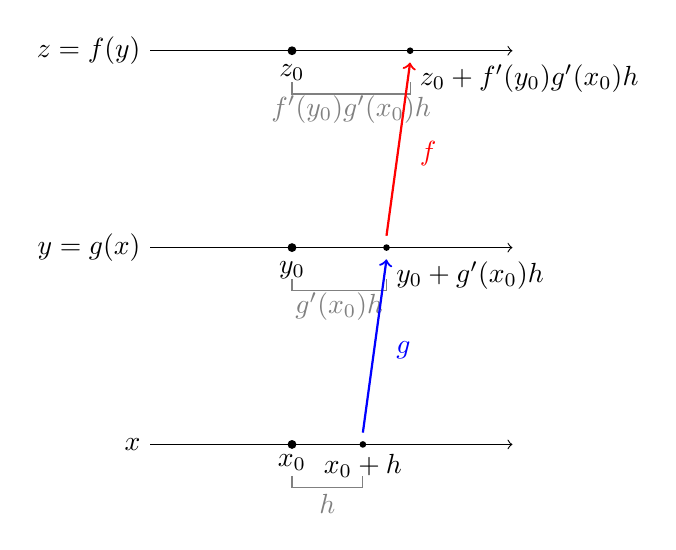
\begin{tikzpicture}[scale=1.0]
% Three horizontal axes
\foreach \k/\lab/\pos in {0/$x$/0, 1/$y = g(x)$/2.5, 2/$z = f(y)$/5} {
  \draw[->] (-0.3,\pos) -- (4.3,\pos);
  \node[left] at (-0.3,\pos) {\lab};
}
% Mark x_0 on bottom axis
\fill (1.5,0) circle (1.6pt);
\node[below] at (1.5,0) {$x_{0}$};
\fill (2.4,0) circle (1.2pt);
\node[below] at (2.4,0) {$x_{0} + h$};
% Bracket showing h
\draw[gray, thin] (1.5,-0.4) -- (1.5,-0.55) -- (2.4,-0.55) -- (2.4,-0.4);
\node[gray] at (1.95,-0.75) {$h$};
% Mark y_0 = g(x_0) and y_0 + g'(x_0)h on middle axis
\fill (1.5,2.5) circle (1.6pt);
\node[below] at (1.5,2.45) {$y_{0}$};
\fill (2.7,2.5) circle (1.2pt);
\node[below right] at (2.7,2.45) {$y_{0} + g'(x_{0}) h$};
% Bracket showing g'(x_0)h
\draw[gray, thin] (1.5,2.1) -- (1.5,1.95) -- (2.7,1.95) -- (2.7,2.1);
\node[gray] at (2.1,1.75) {$g'(x_{0}) h$};
% Mark z_0 = f(y_0) and z_0 + f'(y_0)g'(x_0)h on top axis
\fill (1.5,5) circle (1.6pt);
\node[below] at (1.5,4.95) {$z_{0}$};
\fill (3.0,5) circle (1.2pt);
\node[below right] at (3.0,4.95) {$z_{0} + f'(y_{0}) g'(x_{0}) h$};
% Bracket showing f'(y_0)g'(x_0)h
\draw[gray, thin] (1.5,4.6) -- (1.5,4.45) -- (3.0,4.45) -- (3.0,4.6);
\node[gray] at (2.25,4.25) {$f'(y_{0}) g'(x_{0}) h$};
% Vertical arrows g and f
\draw[->, blue, thick] (2.4,0.15) -- (2.7,2.35);
\node[blue, right] at (2.7,1.2) {$g$};
\draw[->, red, thick] (2.7,2.65) -- (3.0,4.85);
\node[red, right] at (3.0,3.7) {$f$};
\end{tikzpicture}
\caption{The chain rule in pictures. A small displacement \(h\) at the input is scaled by \(g'(x_{0})\) at the intermediate stage, then scaled again by \(f'(y_{0})\) at the output. The total scaling is the product \(f'(y_{0}) g'(x_{0})\) --- which, written in terms of \(x_{0}\), is \(f'(g(x_{0})) g'(x_{0})\).}
\label{fig:chain-rule-mapping}
\end{figure}

% expansion:summary — closing synthesis paragraph linking to §3.3
The chain rule completes the differentiation toolkit for any expression we can build from polynomials, exponentials, sine, cosine, and the four arithmetic operations, plus composition. What remains is a particular set of \emph{indirect} applications: when a function is given implicitly through a relation like \(\sin(\arcsin y) = y\) or \(e^{\ln x} = x\), the chain rule applied to both sides produces the derivative of the implicitly-defined function, even when an explicit formula is hard to extract. The next section uses this technique to compute \(d/dx \ln x\), \(d/dx \arcsin y\), and \(d/dx x^{x}\), each of which would otherwise require its own ad-hoc argument.

\section{Applications of the Chain Rule}\label{sec:chain-rule-applications}

% expansion:intuition — section opener pivoting from §3.2's preview "indirect applications via implicit relations"
The chain rule is the universal tool for differentiating compositions, but its real power emerges when we apply it not to an explicit composition like \(\sin(x^{2})\) but to a defining identity like \(e^{\ln x} = x\). Differentiating both sides of such an identity by the chain rule produces an equation involving the derivative we want, which we can then solve. This technique --- usually called \emph{implicit differentiation} or \emph{logarithmic differentiation} when a logarithm is involved --- delivers the derivatives of \(\ln x\), \(\arcsin y\), and \(x^{x}\) from a single template, even though none of the three has a difference quotient that simplifies cleanly on its own.

% expansion:caution — ln is used here before rigorous construction in ch04; flag the dependency upfront so readers know the worry
\begin{caution}
Throughout this section we use the natural logarithm \(\ln x\) informally as ``the inverse of \(e^{x}\)'': the function on \((0, \infty)\) satisfying
\[
e^{\ln x} = x \quad \text{for } x > 0, \qquad \ln(e^{x}) = x \quad \text{for } x \in \mathbb{R}.
\]
The rigorous construction of \(\ln\) (as the inverse of the strictly increasing function \(e^{x}\), with continuity proved separately) is deferred to \cref{sec:logarithm}. Treating \(\ln\) informally is justified for the chain-rule derivations below: once the inverse exists and is differentiable, the chain rule extracts its derivative. Whether the inverse exists and is differentiable at all is what the rigorous treatment in Chapter 4 settles.
\end{caution}

\subsection{The derivative of \texorpdfstring{$\ln x$}{ln x}}

The defining identity \(e^{\ln x} = x\) for \(x > 0\) is a composition: \(p(x) = f(g(x)) = x\), where \(g(x) = \ln x\) and \(f(y) = e^{y}\). Differentiating both sides extracts \(g'(x)\).

\begin{theorem}\label{thm:derivative-ln}\index{logarithm!derivative}\index{ln@$\ln$!derivative}
For \(x > 0\), \(\displaystyle \frac{d}{dx} \ln x = \frac{1}{x}\).
\end{theorem}

\begin{proof}
Set \(g(x) = \ln x\) and \(f(y) = e^{y}\), so \(f(g(x)) = e^{\ln x} = x\). Differentiating both sides with respect to \(x\):
\[
\frac{d}{dx}[x] = \frac{d}{dx}\bigl[f(g(x))\bigr].
\]
The left side is \(1\). The right side, by the chain rule (\cref{thm:chain-rule}) and \cref{thm:derivative-of-exp},
\[
\frac{d}{dx}\bigl[f(g(x))\bigr] = f'(g(x)) \cdot g'(x) = e^{\ln x} \cdot g'(x) = x \cdot g'(x).
\]
Therefore \(1 = x \cdot g'(x)\), so \(g'(x) = 1/x\).
\end{proof}

% expansion:caution — the proof assumes ln is differentiable; this assumption is what gets justified rigorously in ch04, but flagging it here is more honest than glossing over it
\begin{caution}
The proof above implicitly assumes that \(\ln\) is differentiable at \(x\) --- otherwise the chain-rule manipulation of \(d/dx[f(g(x))]\) is not yet justified. The chain-rule equation alone shows that \emph{if} \(\ln\) is differentiable, then \(d/dx \ln x = 1/x\); the existence of the derivative needs a separate argument, which uses the continuity of \(e^{x}\) and an inverse-function technique (\cref{sec:logarithm}). Many calculus texts blur this point; we flag it here and resolve it in \cref{thm:ln-derivative-rigorous}.
\end{caution}

\subsection{Logarithmic differentiation: the derivative of \texorpdfstring{$x^{x}$}{x\^{}x}}

Functions of the form \(f(x)^{g(x)}\) --- where both the base and the exponent depend on \(x\) --- are not handled by the power rule (which requires a constant exponent) or by the exponential rule (which requires a constant base). The trick is to take \(\ln\) of both sides and apply chain rule + product rule to the resulting expression. The technique is called \emph{logarithmic differentiation}.

% expansion:strategy — log differentiation is the second-most-useful chain-rule application in calculus (after implicit); naming it as a strategy makes it portable
\begin{strategy}[Logarithmic differentiation]
To differentiate a function \(W(x)\) of the form \(f(x)^{g(x)}\) --- or more generally any expression where taking \(\ln\) simplifies the structure (products of many factors, quotients with several pieces):
\begin{enumerate}
    \item Set \(W = W(x)\) and write \(\ln W = \ln(\text{expression})\); use \(\ln\) properties (\(\ln(fg) = \ln f + \ln g\), \(\ln(f^{g}) = g \ln f\)) to expand.
    \item Differentiate both sides with respect to \(x\). The left side becomes \(W'(x) / W(x)\) by chain rule on \(\ln W(x)\); the right side becomes a sum or product of simpler derivatives.
    \item Solve for \(W'(x)\) by multiplying through by \(W(x)\), substituting back the original expression for \(W\) where convenient.
\end{enumerate}
\end{strategy}

\begin{workedexample}
\begin{example}\label{ex:derivative-x-to-x}
Differentiate \(W(x) = x^{x}\) for \(x > 0\).
\end{example}

\begin{solution}
\emph{Step 1.} Take the natural log:
\[
\ln W(x) = \ln(x^{x}) = x \ln x.
\]

\emph{Step 2.} Differentiate both sides. The left side: by the chain rule,
\[
\frac{d}{dx}[\ln W(x)] = \frac{1}{W(x)} \cdot W'(x) = \frac{W'(x)}{W(x)}.
\]
The right side: by the product rule (\cref{thm:product-rule}) on \(x \cdot \ln x\),
\[
\frac{d}{dx}[x \ln x] = 1 \cdot \ln x + x \cdot \frac{1}{x} = \ln x + 1.
\]

\emph{Step 3.} Equate and solve:
\[
\frac{W'(x)}{W(x)} = \ln x + 1, \qquad W'(x) = (1 + \ln x) \cdot W(x) = (1 + \ln x) x^{x}. \qedhere
\]
\end{solution}
\end{workedexample}

% expansion:example — supplementary log-differentiation example showing the technique on a different shape (a product of many factors). Manuscript has only x^x; one more example makes the strategy box's "more generally" clause concrete.
\begin{workedexample}
\begin{example}
Differentiate \(p(x) = \dfrac{(x^{2} + 1) \sqrt{x}}{(x + 3)^{4}}\) for \(x > 0\) using logarithmic differentiation.
\end{example}

\begin{solution}
Take \(\ln\) and use \(\ln(fg/h) = \ln f + \ln g - \ln h\):
\[
\ln p(x) = \ln(x^{2} + 1) + \tfrac{1}{2} \ln x - 4 \ln(x + 3).
\]
Differentiate both sides:
\[
\frac{p'(x)}{p(x)} = \frac{2x}{x^{2} + 1} + \frac{1}{2x} - \frac{4}{x + 3}.
\]
Multiply through by \(p(x)\):
\[
p'(x) = \frac{(x^{2} + 1) \sqrt{x}}{(x + 3)^{4}} \cdot \left(\frac{2x}{x^{2} + 1} + \frac{1}{2x} - \frac{4}{x + 3}\right).
\]
Differentiating directly via repeated quotient and product rules would also work but produces a much longer calculation; the log-differentiation approach is cleaner here because \(\ln\) splits the product into a sum.
\end{solution}
\end{workedexample}

\subsection{The derivative of \texorpdfstring{$\arcsin$}{arcsin}}

The same chain-rule-on-an-identity technique extracts the derivatives of inverse trigonometric functions. We apply it to \(\arcsin\); the same template gives \(\arccos'\) and \(\arctan'\).

\begin{theorem}\label{thm:derivative-arcsin}\index{arcsin@$\arcsin$!derivative}\index{inverse sine function!derivative}
For \(y \in (-1, 1)\),
\[
\frac{d}{dy} \arcsin y = \frac{1}{\sqrt{1 - y^{2}}}.
\]
\end{theorem}

\begin{proof}
The defining identity is \(\sin(\arcsin y) = y\) for \(y \in [-1, 1]\). Set \(g(y) = \arcsin y\) and \(f(x) = \sin x\), so \(f(g(y)) = y\). Differentiating both sides with respect to \(y\),
\[
1 = \frac{d}{dy}[y] = f'(g(y)) \cdot g'(y) = \cos(\arcsin y) \cdot g'(y).
\]
On the principal interval \(\arcsin y \in [-\pi/2, \pi/2]\), cosine is non-negative, so
\[
\cos(\arcsin y) = \sqrt{1 - \sin^{2}(\arcsin y)} = \sqrt{1 - y^{2}}.
\]
For \(y \in (-1, 1)\) the radical is positive, so
\[
g'(y) = \frac{1}{\cos(\arcsin y)} = \frac{1}{\sqrt{1 - y^{2}}}. \qedhere
\]
\end{proof}

% expansion:caution — endpoint behaviour. The formula 1/√(1-y²) blows up at y = ±1, matching the geometric vertical tangent. Worth flagging as the boundary case for the formula.
\begin{caution}
\Cref{thm:derivative-arcsin} is stated for \(y \in (-1, 1)\) only. At the endpoints \(y = \pm 1\) the formula's denominator vanishes; geometrically, the graph of \(\arcsin\) has a vertical tangent at \(y = \pm 1\), so \(\arcsin'\) does not exist there as a finite number. The same domain restriction applies to \(\arccos'\) (proved by the parallel argument: \(\cos(\arccos y) = y\)) which gives \(d/dy \arccos y = -1/\sqrt{1 - y^{2}}\) for \(y \in (-1, 1)\). \(\arctan'\) is better behaved: the formula \(d/dy \arctan y = 1/(1 + y^{2})\) is valid for every \(y \in \mathbb{R}\).
\end{caution}

% expansion:formula — the parallel formulas for arccos and arctan, derived by the same template. Manuscript only covers arcsin; without the others the section is incomplete relative to ch01's three principal arc-trig functions.
\begin{corollary}\label{cor:arctrig-derivatives}
By the same template applied to the defining identities for arccos and arctan,
\pairdisplay{\frac{d}{dy} \arccos y = -\frac{1}{\sqrt{1 - y^{2}}} \ (y \in (-1, 1)),}{\frac{d}{dy} \arctan y = \frac{1}{1 + y^{2}} \ (y \in \mathbb{R}).}
\end{corollary}

\begin{proof}[Sketch]
For arccos: differentiate \(\cos(\arccos y) = y\). The chain rule gives \(-\sin(\arccos y) \cdot \arccos'(y) = 1\); on the principal interval \([0, \pi]\), sine is non-negative, so \(\sin(\arccos y) = \sqrt{1 - y^{2}}\), and \(\arccos'(y) = -1/\sqrt{1 - y^{2}}\).

For arctan: differentiate \(\tan(\arctan y) = y\). The chain rule gives \(\sec^{2}(\arctan y) \cdot \arctan'(y) = 1\), and the identity \(1 + \tan^{2} = \sec^{2}\) gives \(\sec^{2}(\arctan y) = 1 + y^{2}\). Therefore \(\arctan'(y) = 1/(1 + y^{2})\).
\end{proof}

% expansion:summary — closing synthesis paragraph for the chapter, transitioning to ch04
The chain rule and its applications complete the differentiation toolkit for the elementary functions of one variable. Together with the rules of Chapter 2, we can now differentiate every expression built from polynomials, the exponential and logarithmic functions, the trigonometric and inverse trigonometric functions, and any composition, product, quotient, sum, or constant multiple of these. What remains for Chapter 4 is to ground the exponential and logarithmic stories rigorously: define \(e^{x}\) by its power series, prove that \(e^{x}\) is continuous and satisfies the exponent law \(e^{x} \cdot e^{y} = e^{x + y}\), recover its derivative more carefully, and then construct \(\ln x\) as the inverse of \(e^{x}\) with the strict-monotonicity step delivered by the Mean Value Theorem. The chain-rule derivation \(d/dx \ln x = 1/x\) we used above will be re-derived in Chapter 4 from the inverse-function relation directly, without circularity.

\section*{Summary}\addcontentsline{toc}{section}{Summary}

% expansion:summary — chapter-end Summary required by CONTENT_SPEC §4. Items are one-line distillations matching the spec's "different depth, different framing" rule.
\paragraph{Trigonometric derivatives.}
\begin{itemize}
    \item \(\displaystyle \lim_{\theta \to 0} \sin \theta / \theta = 1\), proved by sandwiching with the sector-area inequality \(\sin \theta \leq \theta \leq \tan \theta\) and the squeeze theorem.
    \item \(\sin x\) and \(\cos x\) are continuous on \(\mathbb{R}\); the bound \(\lvert \sin \theta \rvert \leq \lvert \theta \rvert\) drives the proof.
    \item \(\frac{d}{dx} \sin x = \cos x\), \(\frac{d}{dx} \cos x = -\sin x\); by the quotient rule, \(\frac{d}{dx} \tan x = \sec^{2} x\).
\end{itemize}

\paragraph{The chain rule.}
\begin{itemize}
    \item \(p(x) = f(g(x))\) is differentiable wherever \(g\) is differentiable at \(x\) and \(f\) is differentiable at \(g(x)\), with \(p'(x) = f'(g(x)) \cdot g'(x)\). Leibniz form: \(\frac{dz}{dx} = \frac{dz}{dy} \cdot \frac{dy}{dx}\).
    \item Equivalent definitions of differentiability: standard limit form (Def 1, \cref{def:derivative-at-a}) and remainder form (Def 2, \cref{def:differentiable-remainder}).
    \item Proof technique: substitute the remainder-form expansion of \(g\) into the remainder-form expansion of \(f\); the cross-terms collect into a single remainder \(R_{3}(h)\) with \(R_{3}/h \to 0\).
    \item Strategy: identify the outermost operation, differentiate at the abstract argument, multiply by the inner derivative; iterate for nested compositions.
\end{itemize}

\paragraph{Applications of the chain rule.}
\begin{itemize}
    \item \(\frac{d}{dx} \ln x = 1/x\) for \(x > 0\), via chain rule on \(e^{\ln x} = x\) (rigorous construction of \(\ln\) deferred to Ch 4).
    \item Logarithmic differentiation: take \(\ln\) of both sides, differentiate, solve for \(W'\). Yields \(\frac{d}{dx} x^{x} = (1 + \ln x) x^{x}\) and similar formulas for \(f(x)^{g(x)}\).
    \item Inverse-trig derivatives: \(\arcsin'(y) = 1/\sqrt{1 - y^{2}}\), \(\arccos'(y) = -1/\sqrt{1 - y^{2}}\) on \((-1, 1)\); \(\arctan'(y) = 1/(1 + y^{2})\) on \(\mathbb{R}\). Proved via chain rule on the defining identities \(\sin(\arcsin y) = y\) etc.
\end{itemize}

\subsection*{Exercises}

% expansion:summary — exercise inventory deferred per CONTENT_SPEC. Real exercises come from the manuscript; this placeholder respects the Mode A "do not invent exercises" rule.
\emph{Exercises for this chapter are drawn from the manuscript and are deferred to the dedicated exercise pass; see \texttt{CONTENT\_EXERCISES.md}.}

